% =============================================================================
%  ACTIVIDAD — Diseña el sistema antes de construirlo
%  Materia de Verano: Internet of Things (IoT)
%  Universidad Panamericana · Ingeniería Mecatrónica · 6.° semestre
% =============================================================================

\documentclass[11pt, letterpaper]{article}

\usepackage[utf8]{inputenc}
\usepackage[T1]{fontenc}
\usepackage{geometry}
\usepackage{xcolor}
\usepackage{fancyhdr}
\usepackage{titlesec}
\usepackage{enumitem}
\usepackage{parskip}
\usepackage{mdframed}
\usepackage{booktabs}
\usepackage{array}
\usepackage{colortbl}
\usepackage{amssymb}
\usepackage{pgffor}
\usepackage{tikz}
\usepackage{hyperref}
\usepackage{float}
\usepackage[spanish]{babel}          % Idioma español (índice, fechas, etc.)
\usetikzlibrary{arrows.meta, positioning}

\geometry{top=2.2cm, bottom=2.2cm, left=2.5cm, right=2.5cm}
\setlength{\headheight}{22pt}

% ── Colores ───────────────────────────────────────────────────────────────────
\definecolor{upBlue}    {HTML}{2E3A59}
\definecolor{roseMain}  {HTML}{C2547A}
\definecolor{roseLight} {HTML}{FAE8EF}
\definecolor{tealMain}  {HTML}{0F6E56}
\definecolor{tealLight} {HTML}{E1F5EE}
\definecolor{amberMain} {HTML}{854F0B}
\definecolor{amberLight}{HTML}{FAEEDA}
\definecolor{purpleMain}{HTML}{534AB7}
\definecolor{purpleLight}{HTML}{EEEDFE}
\definecolor{grayLight} {HTML}{F5F5F5}
\definecolor{grayMid}   {HTML}{BBBBBB}

% ── Estilos de sección ────────────────────────────────────────────────────────
\titleformat{\section}
  {\large\bfseries\color{upBlue}}{\thesection.}{0.5em}{}
  [\color{roseMain}\titlerule]

\titleformat{\subsection}
  {\normalsize\bfseries\color{upBlue}}{\thesubsection.}{0.5em}{}

% ── Encabezado ────────────────────────────────────────────────────────────────
\pagestyle{fancy}
\fancyhf{}
\fancyhead[L]{\small\color{upBlue} Actividad --- Dise\~na el sistema antes de construirlo}
\fancyhead[R]{\small\color{upBlue} Universidad Panamericana}
\fancyfoot[C]{\small\color{gray}\thepage}
\renewcommand{\headrulewidth}{0.4pt}
\renewcommand{\headrule}{%
  \hbox to\headwidth{\color{roseMain}\leaders\hrule height\headrulewidth\hfill}}

% ── Cajas ─────────────────────────────────────────────────────────────────────
\newenvironment{instruccion}{%
  \begin{mdframed}[backgroundcolor=tealLight, linecolor=tealMain, linewidth=1pt,
    innerleftmargin=10pt, innerrightmargin=10pt,
    innertopmargin=6pt,  innerbottommargin=6pt]
  \small\textbf{\color{tealMain}Instrucci\'on:}\hspace{4pt}
}{\end{mdframed}}

\newenvironment{contexto}{%
  \begin{mdframed}[backgroundcolor=roseLight, linecolor=roseMain, linewidth=1.5pt,
    innerleftmargin=12pt, innerrightmargin=12pt,
    innertopmargin=8pt,  innerbottommargin=8pt]
}{\end{mdframed}}

\newenvironment{cierre}{%
  \begin{mdframed}[backgroundcolor=amberLight, linecolor=amberMain, linewidth=1pt,
    innerleftmargin=10pt, innerrightmargin=10pt,
    innertopmargin=6pt,  innerbottommargin=6pt]%
  \bfseries\color{amberMain}%
}{\end{mdframed}}

% ── Líneas de respuesta ───────────────────────────────────────────────────────
\newcommand{\linea}[1][5cm]{\underline{\hspace{#1}}}
\newcommand{\respuesta}[1]{%
  \vspace{4pt}%
  \foreach \i in {1,...,#1}{%
    \noindent\textcolor{grayMid}{\rule{\linewidth}{0.3pt}}\\[10pt]%
  }%
}


% =============================================================================
\begin{document}
% =============================================================================

% ── Encabezado del documento ──────────────────────────────────────────────────
\begin{center}
  {\color{upBlue}\rule{\linewidth}{1.5pt}}\\[0.3cm]
  {\Large\bfseries\color{upBlue} Actividad}\\[0.2cm]
  {\large\bfseries\color{roseMain}
    Dise\~na el sistema antes de construirlo}\\[0.15cm]
  {\normalsize Materia de Verano: Internet of Things (IoT)
    $\cdot$ Ingenier\'ia Mecatr\'onica $\cdot$ 6.\textdegree\ semestre}\\[0.3cm]
  {\color{roseMain}\rule{\linewidth}{0.8pt}}
\end{center}

\vspace{0.3cm}

\begin{tabular}{rl rl}
  \textbf{Alumno 1:}  & Marco Alberto Vázquez Preciado&
  \textbf{Alumno 2:}  & Jaime Valencia Rodriguez\\[0.5em]
  \textbf{Equipo \#:} & 4&
  \textbf{Fecha:}     & \today      \\
\end{tabular}

\vspace{0.4cm}

\begin{contexto}
  \textbf{\color{roseMain}Contexto:}\\[0.3em]
  Antes de escribir una sola l\'inea de c\'odigo, un equipo de ingenier\'ia siempre
  documenta qu\'e va a construir. Tienen \textbf{25 minutos} para hacer exactamente eso.
  El proyecto que dise\~nan hoy es el mismo que van a implementar durante las
  Semanas~2~y~3: un sistema IoT para controlar y monitorear un motor DC de forma remota
  desde una plataforma web.\\[0.5em]
  \textbf{No busquen en internet.} Usen lo que ya saben.
\end{contexto}

\vspace{0.3cm}

% =============================================================================
\section{Parte A --- Diagrama de bloques del sistema (10 min)}
% =============================================================================

\begin{instruccion}
  Dibujen el sistema completo usando los bloques de abajo como gu\'ia.
  Tracen flechas entre los bloques e indiquen qu\'e dato viaja en cada flecha
  (nombre del dato, no solo una l\'inea). El bloque central del protocolo
  l\'o dejan con \textbf{?} --- lo van a definir m\'as tarde.
\end{instruccion}

\vspace{0.5cm}

% ── Diagrama base con TikZ ────────────────────────────────────────────────────
\begin{figure}[H]
   \centering
   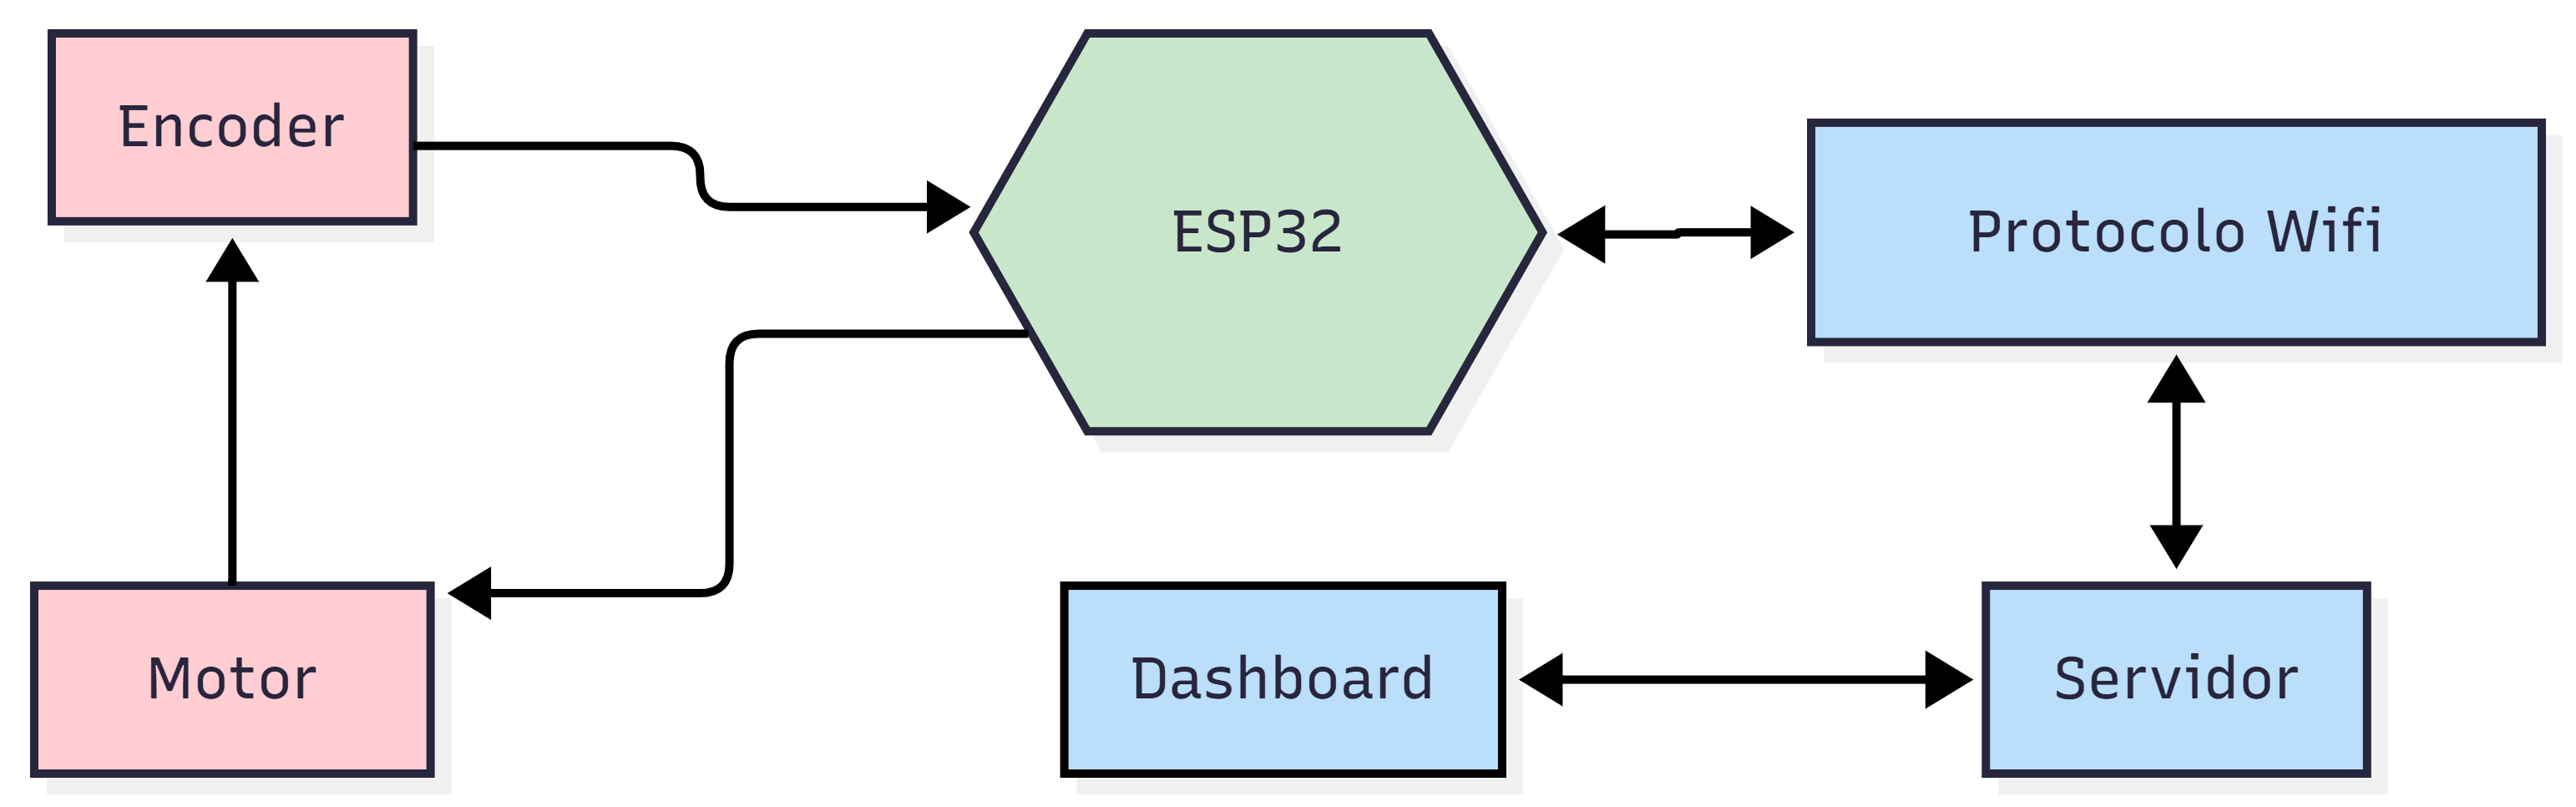
\includegraphics[width=0.85\textwidth]{FlowChart.png}
   \caption{Diagrama de conexiones}
   \label{fig:serial}
 \end{figure}

\vspace{0.5cm}

\subsection{Describe qu\'e hace cada bloque}

\begin{tabular}{>{\bfseries\color{upBlue}}p{3.2cm}
                p{5.5cm} p{5.5cm}}
  \toprule
  \textbf{Bloque} &
  \textbf{Qu\'e hace} &
  \textbf{Qu\'e datos env\'ia / recibe} \\
  \midrule
  Encoder / Sensor   & Lee el valor RPM del motor& NOTIFY\\[1.6em]
 Motor& Girar&NA\\
  ESP32 (Motor)      & Recibir el valor leído de RPM y generar un valor PWM para modificar al motor y hacer el cálculo de PID para permitir un control adecuado& NOTIFY \& READ / WRITE\\[1.6em]
  Protocolo (?)      & Permite el intercambio de datos entre el ESP32 y el servidor& TRANSMISIÓN\\[1.6em]
  Servidor / Gateway & Puente entre la ESP32 y el dashboard que sirve como nube donde se procesan los datos para ser mostrados a los usuarios& ENRUTADOR\\[1.6em]
  Dashboard Web      & Interacción directa del usuario hacia el sistema donde es capaz de definir nuevas velocidades y visualizar la información esencial del motor& WRITE / NOTIFY\\[1.6em]
  \bottomrule
\end{tabular}

\newpage

% =============================================================================
\section{Parte B --- Las tres preguntas de decisi\'on (10 min)}
% =============================================================================

\begin{instruccion}
  Respondan sin buscar en internet. Usen lo que ya saben de la clase de hoy y del
  D\'ia~2. Al final escriban una \textbf{conclusi\'on provisional} --- no importa
  si cambia despu\'es, lo que importa es que tengan un argumento t\'ecnico.
\end{instruccion}

\vspace{0.3cm}

% ── Pregunta 1 ────────────────────────────────────────────────────────────────
\subsection{%
  \texorpdfstring{%
    \textcolor{roseMain}{1}~~%
    \textquestiondown A cu\'antos metros est\'a el motor del servidor?%
  }{Pregunta 1}%
}

En el escenario de la f\'abrica, estima una distancia realista.
\textit{(Pista: una planta manufacturera mediana puede tener entre 50 m y 2~km de largo.)}

\vspace{0.2cm}
\textbf{Distancia estimada:} 100m
\hspace{1cm}
\textbf{?`Qu\'e protocolo favorece esa distancia?} Wi-Fi

\vspace{0.2cm}
\textbf{Justificaci\'on breve:} Al ser una distancia relativamente corta, podemos utilizar WiFi para tener una mayor velocidad de envio de datos.

% ── Pregunta 2 ────────────────────────────────────────────────────────────────
\subsection{%
  \texorpdfstring{%
    \textcolor{roseMain}{2}~~%
    \textquestiondown El nodo del motor tiene bater\'ia o cable de corriente?%
  }{Pregunta 2}%
}

\begin{tabular}{ll}
  \textbf{Elecci\'on:} &
  $\square$~Bater\'ia \quad $\boxtimes$~Cable de corriente \quad
  $\square$~Depende del caso \\[0.6em]
\end{tabular}

\textbf{?`Qu\'e implica esto para el consumo del protocolo de comunicaci\'on?}
Esto provoca que no nos importe mucho el consumo de energia de nuestro protocolo de comunicacion ya que estamos conectados directamente a la corrinte y no tenemos que administrar el almacenamiento de la bateria.

% ── Pregunta 3 ────────────────────────────────────────────────────────────────
\subsection{%
  \texorpdfstring{%
    \textcolor{roseMain}{3}~~%
    \textquestiondown Cu\'antos bytes por segundo necesita transmitir el sistema?%
  }{Pregunta 3}%
}

El payload m\'inimo de un paquete de telemetr\'ia es:

\begin{center}
\begin{tabular}{lcr}
  \toprule
  \textbf{Campo}          & \textbf{Tipo}    & \textbf{Tama\~no} \\
  \midrule
  RPM real                & \texttt{float}   & 4 bytes \\
  Setpoint actual         & \texttt{float}   & 4 bytes \\
  Timestamp (\texttt{ms}) & \texttt{uint32}  & 4 bytes \\
  ID del nodo             & \texttt{uint8}   & 1 byte  \\
  Status                  & \texttt{uint8}   & 1 byte  \\
  \midrule
  \textbf{Total}          &                  & \textbf{14 bytes}\\
  \bottomrule
\end{tabular}
\end{center}

\vspace{0.3cm}

\textbf{?`Cada cu\'anto tiempo env\'ian un paquete?}
\hspace{0.5cm}
$\square$~Cada 200~ms \quad
$\square$~Cada 500~ms \quad
$\square$~Cada 2~s \quad
$\boxtimes$~Otro: 100 ms

\vspace{0.3cm}

\textbf{Bytes por segundo resultantes:} 140 bytes/s
\hspace{0.5cm}
\textbf{?`Requiere mucho ancho de banda?} No

% ── Conclusión provisional ────────────────────────────────────────────────────
\vspace{0.3cm}
\begin{mdframed}[backgroundcolor=purpleLight, linecolor=purpleMain, linewidth=1.5pt,
  innerleftmargin=12pt, innerrightmargin=12pt,
  innertopmargin=8pt,  innerbottommargin=8pt]
  \textbf{\color{purpleMain}Conclusi\'on provisional del equipo:}\\[0.5em]
  \textit{Creemos que deber\'iamos usar}
  \underline{WiFi}
  \textit{porque\ldots}\\[0.4em]
  Estamos transmitiendo datos a una distancia relativamente corta, y a una alta velocidad. Ademas, como contamos con una toma de corriente, nos podemos dar el lujo de usar un protocolo que consuma mucha energia pero que nos entregue datos de forma casi inmediata.
  \small\textit{(Esta decisi\'on puede cambiar cuando veamos el tema de hoy.
  Lo importante es que tengan un argumento, no que sea la respuesta correcta.)}
\end{mdframed}

\newpage

% =============================================================================
\section{Parte C --- Pregunta técnica (5 min)}
% =============================================================================

\begin{instruccion}
  Cada equipo escribe \textbf{una sola pregunta t\'ecnica} que tienen sobre el proyecto
  y que no saben responder todav\'ia. Debe ser espec\'ifica --- no
  ``\textit{?`c\'omo funciona LoRa?}'' sino algo como
  ``\textit{?`Si el PID corre en el ESP32 y se cae el WiFi, el motor sigue
  funcionando?}''. Entreguen esta hoja al profesor al terminar.
\end{instruccion}

\vspace{0.5cm}

\textbf{Nuestra pregunta:}
¿Qu\'e sucede si se pierde conexión al servidor por parte de la ESP? ¿qué consecuencias tendría esto con el motor y su velocidad? ¿desde dónde retomaría su función al reconectarse?

\vspace{0.5cm}

\textbf{?`Por qu\'e esa pregunta es importante para el dise\~no del sistema?}
Porque al ser un entorno industrializado y real los errores y fallos deben suponerse posibles, y como ingenieros se deben tener planes de contingencia ante estos posibles cambios, diganse desconexiones o fluctuaciones en la energía son variables posibles que afecten el sistema.

\vspace{1cm}

% ── Lista de verificación ─────────────────────────────────────────────────────
\begin{mdframed}[backgroundcolor=amberLight, linecolor=amberMain, linewidth=1pt,
  innerleftmargin=12pt, innerrightmargin=12pt,
  innertopmargin=8pt,  innerbottommargin=8pt]
  \textbf{\color{amberMain}Antes de entregar --- verifiquen:}
  \begin{itemize}[leftmargin=1.5cm, label=$\boxtimes$, itemsep=2pt]
    \item El diagrama de bloques tiene flechas con el nombre del dato en cada una
    \item La tabla de bloques tiene al menos una oraci\'on por celda
    \item Las tres preguntas de la Parte~B tienen respuesta escrita (aunque sea breve)
    \item La conclusi\'on provisional tiene un argumento t\'ecnico, no de preferencia
    \item La pregunta de la Parte~C es espec\'ifica y relevante al proyecto
  \end{itemize}
\end{mdframed}

\end{document}
